%%%%%%%%%%%%%%%%%%%%%%%%%%%%%%%%%%%%%%%%%%%%%%%%%%%%%%%%%%%%%%%%%
%%% COSYNE-2007 Abstract Template
%%% Version 1.0
%%%%%%%%%%%%%%%%%%%%%%%%%%%%%%%%%%%%%%%%%%%%%%%%%%%%%%%%%%%%%%%%%
%
%http://www.cosyne.org/c/index.php?title=Abstracts
%
%Submission Format
%
%Before you log onto the submission website, you should have the following items prepared: (1) title, (2) author list (including email addresses of all authors), and (3) two-page PDF submission. Submissions that do not meet the following guidelines may be rejected.
%
%Abstracts will be evaluated on the basis of a two page (A4 or US Letter) submission in PDF format. This two-page PDF should contain:
%
%    Title - 100 characters or fewer (including spaces), capitalized in sentence case
%    300-word Summary - brief description of the study's primary findings, emphasizing their significance, generality, novelty and relevance. You will be asked to copy this 300-word summary into a text-only box; it will be included in the conference program if your submission is accepted.
%    Additional Detail - use the remaining space to expand upon the central question(s), approach, results, and/or conclusions of the study. You may include equations as appropriate. Figures are optional. You need not touch upon all the major points of the Summary, but should aim to include whatever detail will best help reviewers to evaluate the significance of your study. Do not feel obliged to fill the entire two pages.
%    Double-blind - The reviewing process for Cosyne will be double blind at the level of reviewers. Authors are responsible for anonymizing their submission. In particular, do not include author names, author affiliations, or acknowledgements in the abstract or body of the submission and avoid providing any other identifying information in text or figures. If you need to cite one of your own publications, you should do so with adequate anonymization to preserve double-blind reviewing (e.g., write “In the previous work of Author et al. [1]…” rather than “In our previous work [1]...”). If you need to cite one of your own papers that is a non-anonymous preprint (on arXiv, social media, websites, etc.) please do so with adequate anonymization (e.g., if the cited submission is available as a non-anonymous preprint, then write “Author et al. [1] concurrently show…”). Reviewers will be instructed not to actively look for such preprints, but encountering them will not constitute a conflict of interest. Alternatively, authors may submit work that is already available as a preprint (e.g., on arXiv) without citing it; however, previously published papers by the authors on related topics must be cited (with adequate anonymization to preserve double-blind reviewing). 
%
%Font size (including any figure legends) must be at least 12 point. Margins should be at least 0.5". This two-page PDF will be the only document seen by reviewers. (Abstracts exceeding two pages will have additional pages removed). Submissions that do not meet these guidelines may be rejected.
%
%For questions regarding abstract submission, please contact: meeting [at] cosyne.org
%
%
%Evaluation Criteria
%
%PDF submissions will be evaluated on the basis of the following criteria:
%
%    Significance
%    Originality
%    Clarity
%    Relevance to the Cosyne audience. 
%
%The submission should clearly explain why your question is important and how your claims will advance the field. Include enough detail that reviewers can assess the technical content of your methods and results. Please be sure to address the significance and fit of your submission for the Cosyne audience, which includes a mix of experimentalists and theoreticians interested in the functional properties of neural systems. Potentially inappropriate abstracts include pure machine learning studies, or studies of single cells with no clear implications for neural systems.
%
%Approximately 30 submissions will be chosen for short talks and ~330 will be chosen for poster presentations. 
%

%\documentclass[12pt,draft]{article}
\documentclass[12pt]{article}
\usepackage{times}
%\inner 0.5in
\oddsidemargin -0.5in		% margin, in addition to 1" standard
\textwidth 7.5in		% 8.5" - 2*(1+\oddsidemargin)

\topmargin -1in		% in addition to 1.5" standard margin
\textheight 9.75in 		% 11 - ( 1.5 + \topmargin + <bottom-margin> )

\columnsep 0.25in

\parindent 0pt
\parskip 12pt

\flushbottom \sloppy
\pagestyle{empty} % No page numbers

\usepackage{subfigure}
\usepackage{tikz}
\usepackage{csquotes}
\usepackage{caption}
%\usepackage{floatrow}
%\usepackage[footnotesize]{caption}

\usepackage[
%style=chem-acs,
style=numeric,						% numeric style for reference list
citestyle=numeric-comp,
%style=alphabetic-verb,
giveninits=false,
maxbibnames=1,
firstinits=true,
%style=apa,
%maxcitenames=1,
%maxnames=3,
%minnames=1,
%maxbibnames=99,
dateabbrev=true,
giveninits=true,
%uniquename=init,
url=false,
doi=false,
isbn=false,
eprint=false,
texencoding=utf8,
bibencoding=utf8,
autocite=superscript,
backend=biber,
%sorting=none,
sorting=nty,
sortcites=false,
%articletitle=false
]{biblatex}%
\newcommand{\citep}[1]{\parencite{#1}}
\newcommand{\citet}[1]{\textcite{#1}}
\bibliography{biblio.bib} % the ref.bib file

\usepackage{wrapfig}
\usepackage{siunitx}
%\renewcommand{\cite}{\citep}%
\newcommand{\ms}{\si{\milli\second}}%

%%%%%%%%%%% BEGIN METADATA %%%%%%%%%%%%
\newcommand{\AuthorAG}{Antoine Grimaldi}

\newcommand{\AuthorLP}{Laurent Perrinet}
\newcommand{\AuthorVB}{Victor Boutin}
\newcommand{\AddressLP}{Institut de Neurosciences de la Timone (UMR 7289); Aix Marseille Univ, CNRS; Marseille, France}%
\newcommand{\WebsiteLP}{https://laurentperrinet.github.io}%
\newcommand{\EmailLP}{Laurent.Perrinet@univ-amu.fr}%
\newcommand{\EmailRB}{xxx@xxx}%
\newcommand{\AuthorSI}{Sio-Hoi Ieng}
\newcommand{\AuthorRB}{Ryad Benosman}%
\newcommand{\orcidRB}{0000-0003-0243-944X}%
\newcommand{\AddressRB}{Sorbonne Université, INSERM, CNRS, Institut de la Vision, France;}%
\newcommand{\Summary}{ % TIP: depuis la PDF, je copie le summary et lance  "pbpaste |wc -w" -------->  285 mots
%Reverse engineering is the art of looking at an existing device in order to understand its concepts and operation. 
%We used this approach to link innovative methods used in computer vision to computational neuroscience. 
We propose a neuromimetic Spiking Neural Network (SNN) architecture able to perform pattern recognition. % in an end-to-end event-based way. 
To achieve this, we extended the algorithm presented in~\citet{Lagorce17}, an event-based algorithm which introduced novel spatio-temporal features: time-surfaces. Built from asynchronous events acquired by a neuromorphic camera, these time-surfaces allow to code the local dynamics of a visual scene and to create an efficient hierarchical event-based pattern recognition architecture. 
Our work is three-fold. First, through the analysis of this existing method we were able to adapt its formalism in the computational neuroscience domain by drawing an analogy with SNN of leaky integrate-and-fire (LIF) models and Hebbian learning. 
Then, %after reproduction of their results, 
generalization of the classification task with a more complex and widely used dataset (N-MNIST, ~\citet{Orchard15}) was performed using logistic regression. A significant contribution was to achieve online classification of the N-MNIST dataset reaching state of the art performances. To our knowledge, it is the first end-to-end event-based online classification network of this kind. The third contribution came by adding an homeostatic regulation rule inspired by biology for neural activity. According to the efficient coding hypothesis, neural activity should be equally distributed between neurons. We used this principle to force neurons in the same layer to spike on average with balanced firing rates by setting for each neuron a gain depending on their past activity. Efficiency of this technique was demonstrated through an improvement in spatio-temporal patterns which were learned during the training phase and a classification performance reaching $97,8\%$ accuracy. As a summary, %by using a method used in a different field, 
we were able to develop a neuromimetic SNN model for online digit classification. We aim at pursuing the study of this architecture through unsupervised learning of natural scene and hope to offer insights on the efficiency of the processing in neural tissues.
}

\usepackage{titlesec}
% \titlespacing*{<command>}{<left>}{<before-sep>}{<after-sep>}
\titlespacing*{\section}
{0pt}{1.5ex}{0.8ex}
\titlespacing*{\subsection}
{0pt}{0.9ex}{0.4ex}
\titlespacing*{\subsubsection}
{0pt}{0.5ex}{0.3ex}
\titlespacing*{\paragraph}{%
  0pt}{%              left margin
  0.0\baselineskip}{% space before (vertical)
  1em}%               space after (horizontal)

\usepackage{setspace}

\begin{document}

%%%-----------------------------------------------------------------
{\Large\bf
%An end-to-end event-based image classification algorithm using a Spiking Neural Network model
%An 
Event-driven Spiking Neural Networks %model 
for
pattern recognition
%  image classification
}

{\bf
Anonymous submission for double-blind review.
%\AuthorAG$^{\dagger}$, \AuthorVB$^{\dagger}$, \AuthorLP$^{\dagger}$, \AuthorSI$^{\ddagger}$ and \AuthorRB$^{\ddagger}$
}
%
%{
%$\dagger$ \AddressLP \\
%$\ddagger$ \AddressRB
%}

%%%-----------------------------------------------------------------
%%SUMMARY
\paragraph*{Summary}
\Summary
%%END OF SUMMARY
%
\begin{wrapfigure}{L}{.7\textwidth}
\vspace{-15pt}
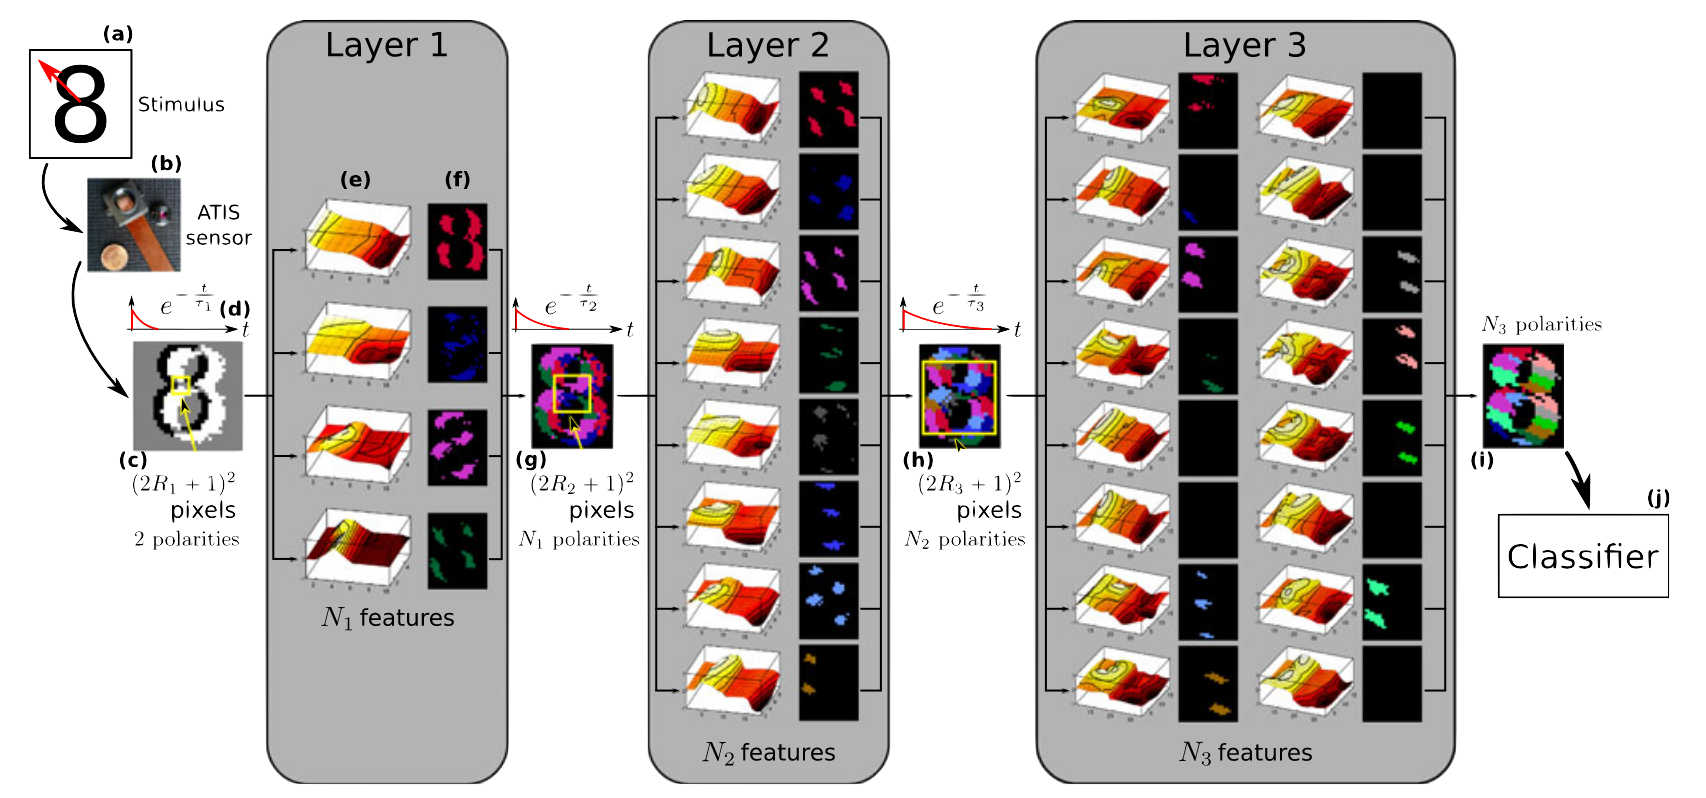
\includegraphics[width=1.04\linewidth]{../notebooks/fig/hots.png}
\vspace{-45pt}
\caption*
{\label{fig:fig1}
}
\end{wrapfigure}


\paragraph*{Figure 1 : }
\textbf{The HOTS algorithm (extracted from~\citep{Lagorce17}).}  
The input of the network is a stream of ON and OFF events (c) $ev_i = [t_i,X_i,p_i]^T$ captured from a moving digit (a) where $t_i$ is the time of the event, $X_i=[x_i,y_i]^T$ its pixel address on the event-based sensor (b) and $p_i$ its polarity. To use spatio-temporal information, ~\citep{Lagorce17} apply an exponential decay (d) to each event. Therefore, at event $ev_k$, the analog value in pixel $X_p$ is $s_p(t_k) = e^\frac{-(t_k-t_{last}(X_p))}{\tau}$ with $t_{last}(p)$ the time recorded for the last event on pixel $p$. In terms of neuronal dynamics, $s_p$ corresponds to the membrane potential evolution of a LIF model. A time-surface $S_k$ gathers $s_i(t_k)$ values for all $i$ within a spatial window surrounding $X_k$. It is compared to the different features (e) of a layer with euclidian distance $ \beta_k = \frac{\langle C_j,S_k\rangle}{\|C_j\|\|S_k\|}$ where $C_j$ is feature number $j$. When a feature gets the smallest euclidian distance with the input, it produces an event in the channel corresponding to the matched feature (f). "Neurons" within the same layer are then spiking in a competitive fashion. Events from the $N_1$ features constitute the output of the layer (g). Each layer takes input from its previous layer and feeds the next by reproducing steps (d)-(g). We can find that $ \beta_k(t) =  \sum_{n=1}^{(2R+1)^2}e^\frac{-(t_i-t_n)}{\tau}c_{kn}$, $R$ being the spatial window parameter of the time-surface and $c_{kn}$ the value stored in feature $k$ at address $n$. In the computational neuroscience framework, $c_{kn}$ represent pre-synaptic weights for neuron $k$ and the hierarchical networks presented in ~\citep{Lagorce17} corresponds to an end-to-end SNN of LIF models. The output (i) of the last layer is then fed to the classifier (j) which will recognize the object in the input.

%\textbf{The HOTS algorithm (extracted from~\citep{Lagorce17}).} The N-MNIST dataset consists of (a) digits presented to (b) the (possibly moving) event-based camera. It produces (c) ON and OFF events which are fed into Layer 1. The events are convolved with exponential kernels (d) to build event contexts from spatial receptive field %of side-length $2R1+1$, 
%known as \emph{time-surfaces}. These time-surfaces are clustered into $N_1$ features (e). When a feature gets the smallest euclidian distance with the input, it produces an event in the channel corresponding to the matched feature (f). Events from the $N_1$ features constitute the output of the layer (g). Each layer takes input from its previous layer and feeds the next by reproducing steps (d)-(g). The output (i) of the last layer is then fed to the classifier (j) which will recognize the object in the input.

%----------------------------------------------


%\begin{figure}
%  \begin{minipage}[c]{0.65\textwidth}
%    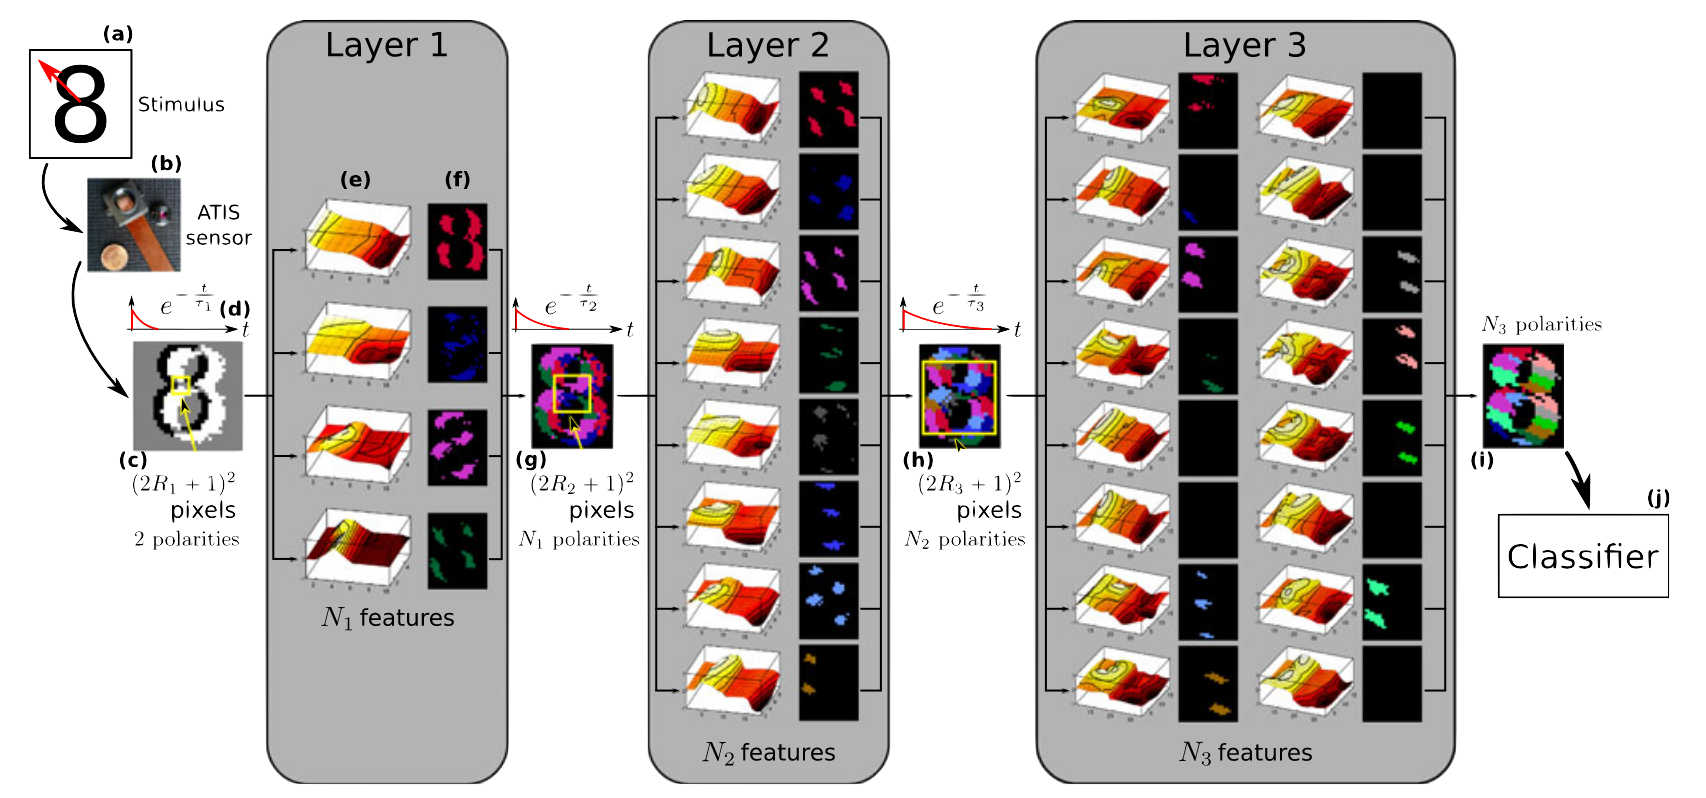
\includegraphics[width=\textwidth]{../notebooks/fig/hots.png}
%  \end{minipage}\hfill
%  \begin{minipage}[c]{0.35\textwidth}
%    \caption{
%\textbf{The HOTS algorithm (extracted from~\citep{Lagorce17}).} The N-MNIST dataset consists of (a) digits presented to (b) the (possibly moving) event-based camera. It produces (c) ON and OFF events which are fed into Layer 1. The events are convolved with exponential kernels (d) to build event contexts from spatial receptive field of side-length $2R1+1$, known as \emph{time-surfaces}. These time-surfaces are clustered into $N_1=4$ features (e). When a feature gets the smallest euclidian distance with the input, it produces an event in the channel corresponding to the matched feature (f). Events from the $N_1=4$ features constitute the output of the layer (g). Each layer takes input from its previous layer and feeds the next by reproducing steps (d)-(g). The output (i) of the last layer is then fed to the classifier (j) which will recognize the object in the input.
%    } \label{fig:fi1}
%  \end{minipage}
%\end{figure}


%\begin{figure}
%\floatbox[{\capbeside\thisfloatsetup{capbesideposition={left,top},capbesidewidth=.2\linewidth}}]{figure}
%{\caption{\textbf{The HOTS algorithm (extracted from~\citep{Lagorce17}).} The N-MNIST dataset consists of (a) digits presented to (b) the (possibly moving) event-based camera. It produces (c) ON and OFF events which are fed into Layer 1. The events are convolved with exponential kernels (d) to build event contexts from spatial receptive field of side-length $2R1+1$, known as \emph{time-surfaces}. These time-surfaces are clustered into $N_1=4$ features (e). When a feature gets the smallest euclidian distance with the input, it produces an event in the channel corresponding to the matched feature (f). Events from the $N_1=4$ features constitute the output of the layer (g). Each layer takes input from its previous layer and feeds the next by reproducing steps (d)-(g). The output (i) of the last layer is then fed to the classifier (j) which will recognize the object in the input.
%}\label{fig:fig1}}
%{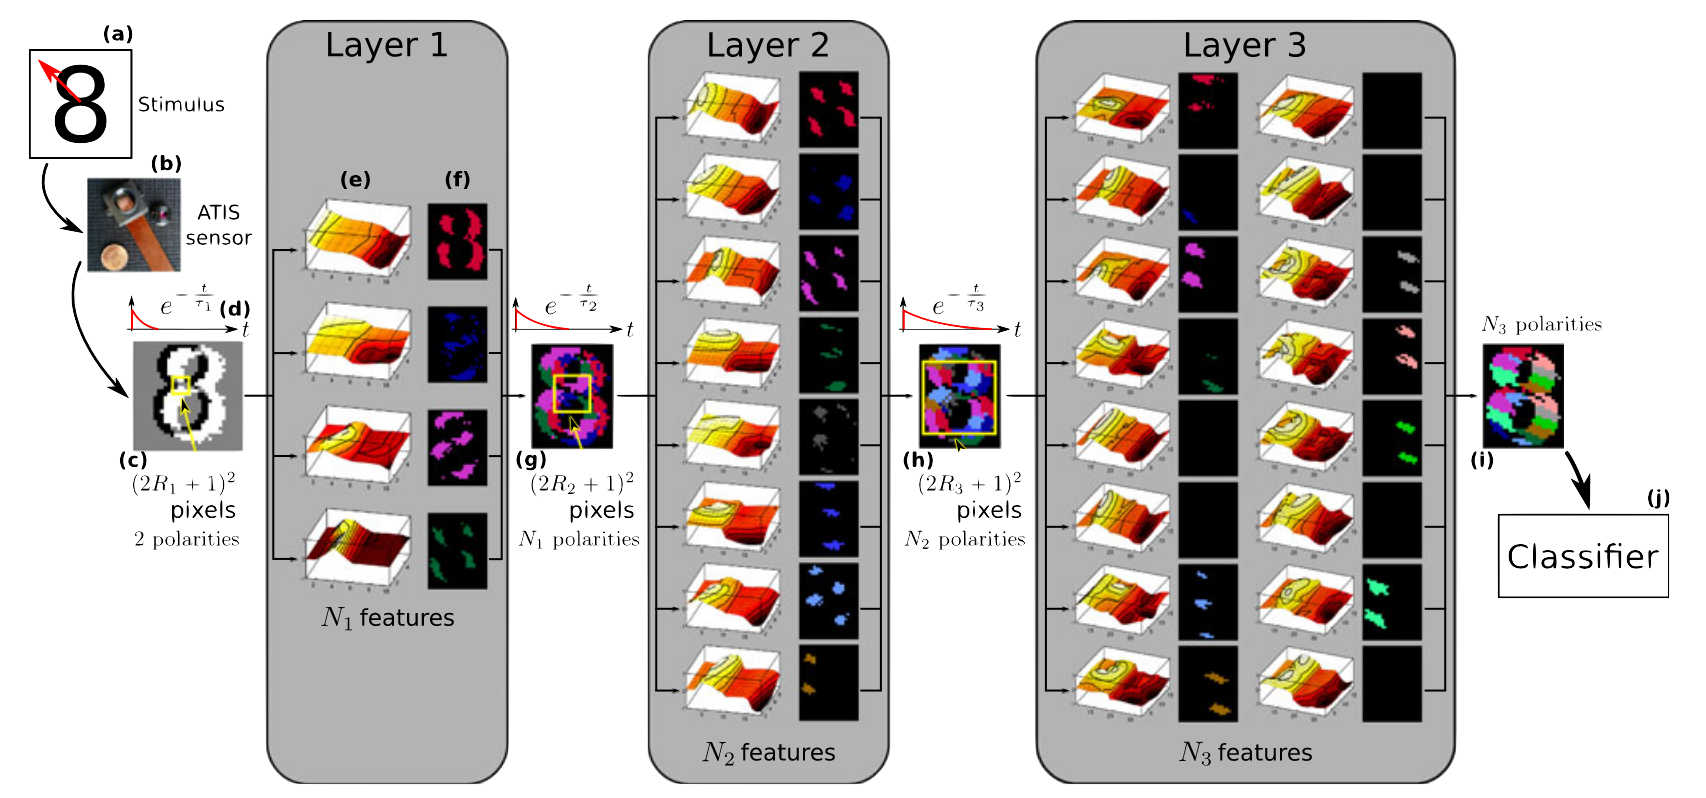
\includegraphics{../notebooks/fig/hots.png}}
%\end{figure}

%\parindent 12pt
%\begin{figure}[!ht]%[!ht][!b]%
%\begin{figure}{R}{.5\textwidth}
%\floatbox[{\capbeside\thisfloatsetup{capbesideposition={right,top},capbesidewidth=4cm}}]{figure}[\FBwidth]
%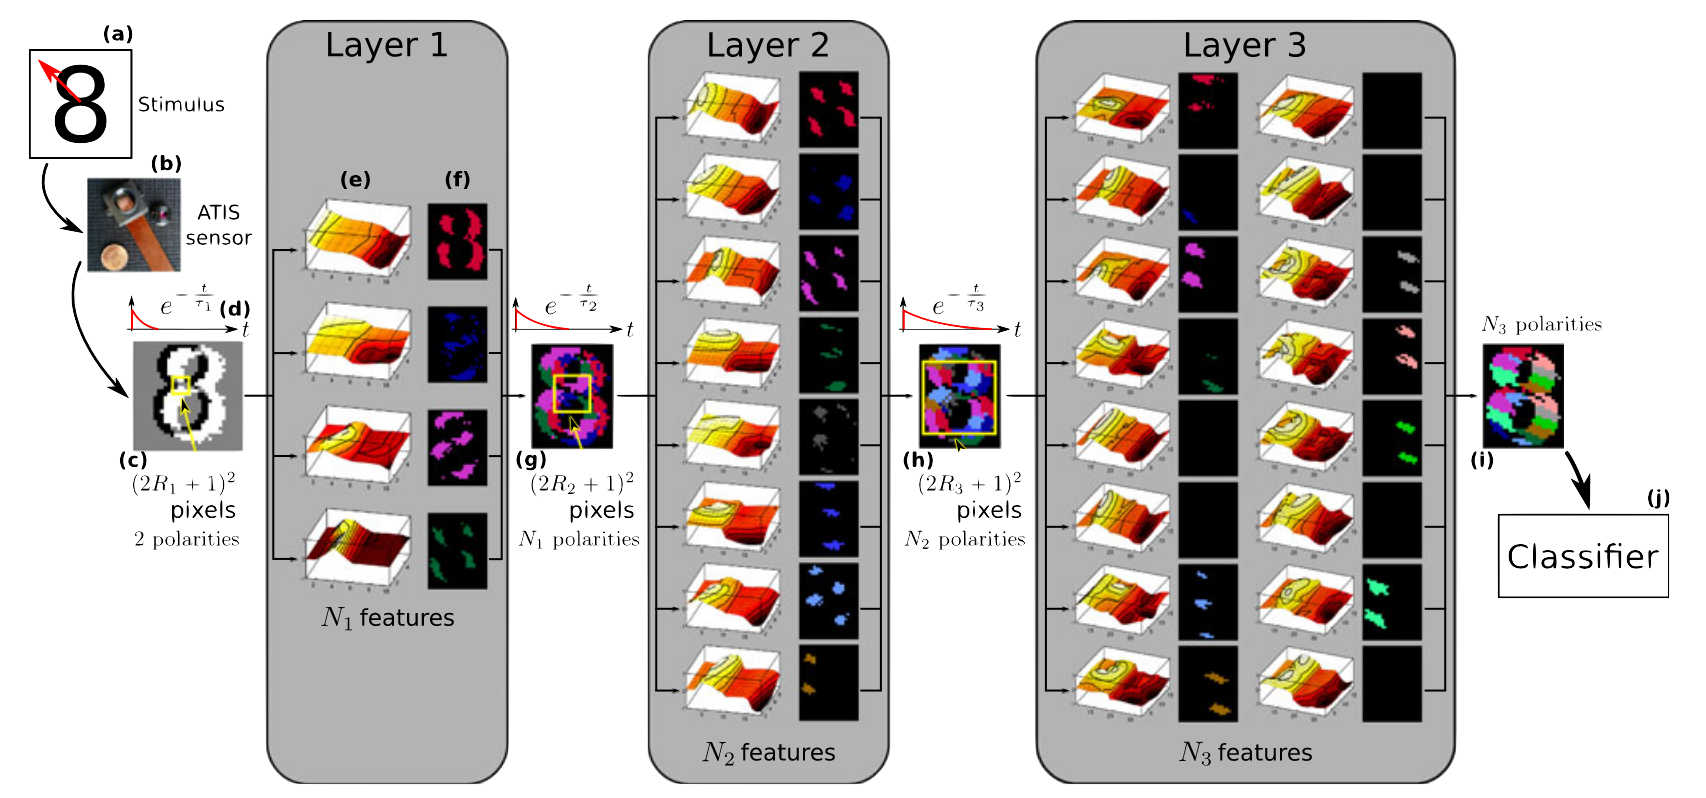
\includegraphics[width=.9\linewidth]{../notebooks/fig/hots.png}
%\caption
%{
%\textbf{The HOTS algorithm (extracted from~\citep{Lagorce17}).} The N-MNIST dataset consists of (a) digits presented to (b) the (possibly moving) event-based camera. It produces (c) ON and OFF events which are fed into Layer 1. The events are convolved with exponential kernels (d) to build event contexts from spatial receptive field %of side-length $2R1+1$, 
%known as \emph{time-surfaces}. These time-surfaces are clustered into $N_1=4$ features (e). When a feature gets the smallest euclidian distance with the input, it produces an event in the channel corresponding to the matched feature (f). Events from the $N_1=4$ features constitute the output of the layer (g). Each layer takes input from its previous layer and feeds the next by reproducing steps (d)-(g). The output (i) of the last layer is then fed to the classifier (j) which will recognize the object in the input.
%\label{fig:fig1}
%}
%\end{figure}
%\end{figure}
%
%\paragraph*{From event-based computing to Spiking Neural Networks}
%The output of an event-based camera is a stream of events $ev_i = [t_i,X_i,p_i]^T$ where $t_i$ is the time of the event, $X_i=[x_i,y_i]^T$ its pixel address and $p_i$ its polarity. In order to use spatio-temporal information, ~\citep{Lagorce17} apply an exponential decay to each event. Therefore, at event $ev_k$, the analog value in pixel $X_p$ is $s_p(t_k) = e^\frac{-(t_k-t_{last}(X_p))}{\tau}$ with $t_{last}(p)$ the time recorded for the last event on pixel $p$. In terms of neuronal dynamics, $s_p$ corresponds to the membrane potential evolution of a LIF model. A time-surface $S_k$ gathers $s_i(t_k)$ values for all $i$ within a spatial window surrounding $X_k$. It is compared to the different features of a layer with euclidian distance $ \beta_k = \frac{\langle C_j,S_k\rangle}{\|C_j\|\|S_k\|}$ where $C_j$ is feature number $j$. We can easily find that $ \beta_k(t) =  \sum_{n=1}^{(2R+1)^2}e^\frac{-(t_i-t_n)}{\tau}c_{kn}$, $R$ being the spatial window parameter of the time-surface and $c_{kn}$ the value stored in feature $k$ at address $n$. In the computational neuroscience framework, $c_{kn}$ represent pre-synaptic weights for neuron $k$ and the hierarchical networks presented in ~\citep{Lagorce17} corresponds to an end-to-end SNN of LIF models. It should be noted that for each event the feature closest to the input spikes. It makes neurons within the same layer spike in a competitive fashion. 
%\begin{figure}[!ht]%[!ht][!b]%

\begin{wrapfigure}{l}{.72\textwidth}
\vspace{-20pt}
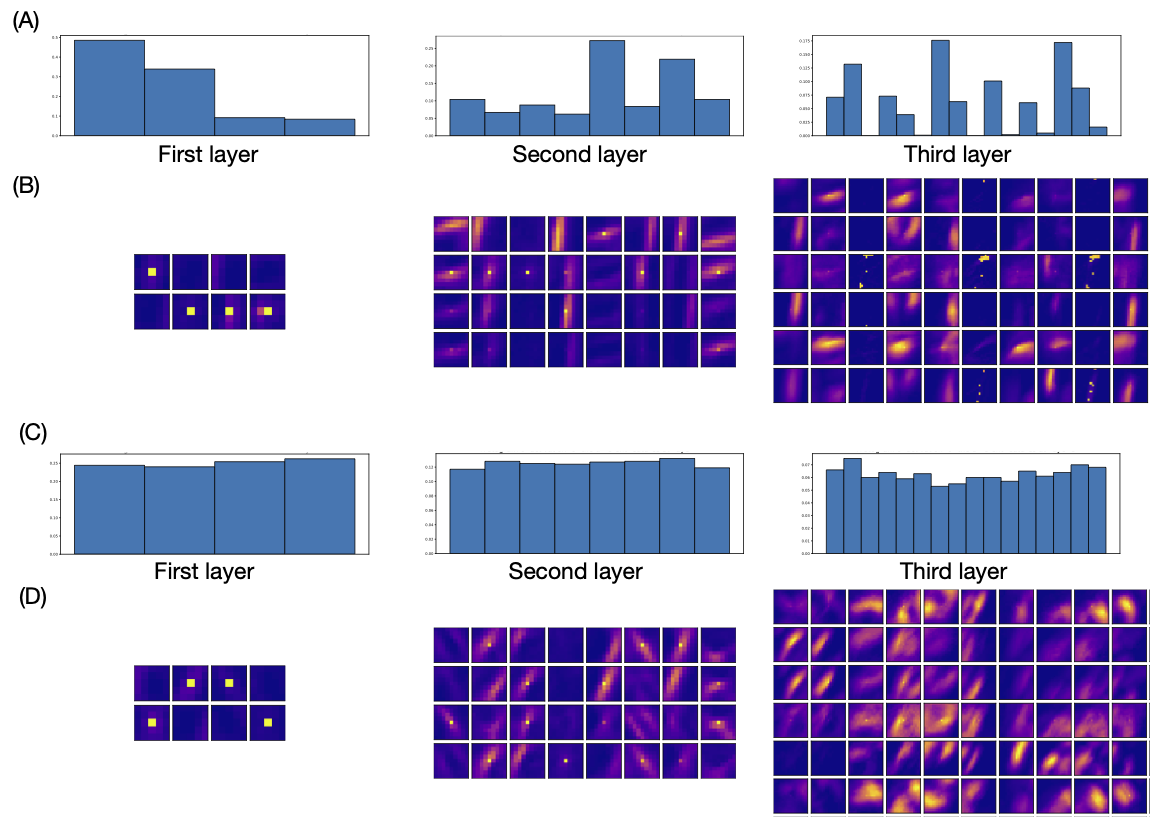
\includegraphics[width=1.03\linewidth]{../layerz.png}
\vspace{-55pt}
\caption*
{
\label{fig:fig2}
}
\end{wrapfigure}

\paragraph*{Figure 2 : }
Activation histograms and features obtained in the self-supervised learning algorithm with (A) and without homeostasis (B). Below histograms are plotted features. The different lines are the different polarities of the features, ON and OFF for the first layer, output channels of the previous layer for the others. In the last layer, only 5 polarities over 8 are display to preserve space and clarity. 

%Features and activation histograms obtained in the self-supervised learning algorithm. (A) and (C) represent the activation histograms for each features within the different layers of the network respectively with and without homeostasis. (B) and (D) are representations of the features learned during the training of the SNN respectively with an without homeostasis. Columns corresponds to the different polarities (ON and OFF for the first layer, output channels of the previous layer for the others) and lines are the features. In the third layer, only 10 features and 6 polarities are presented for the sake of clarity and space use.

%\end{figure}
\paragraph*{Hebbian Learning and the role of homeostasis}
With a simple Hebbian learning rule, see ~\citep{Lagorce17}, neurons learn patterns from spiking input aka time-surfaces in an unsupervised way.
%with the following rule when a feature or neuron $j$ is matched: $C_j \leftarrow C_j + \alpha(S_k-\beta_j C_j)$ where $ \alpha = \frac{0.01}{1+\frac{p_j}{2000}}$, $p_j$ being the number of times feature $j$ was activated. This weight change between neurons refers to Hebbian learning, our network is a simple feedforward SNN with Hebbian learning rule. Neurons will learn patterns from spiking input aka time-surfaces. 
When observing \textit{Figure 2(A)}, we can see that activation of the neurons is unbalanced. It leads to different speeds in learning with unmatured features which are hardly activated. 
%In some cases, learning can lead to grandmother cells and penalize the generalization of the network as well as learning when some neurons are hardly matched. 
In \textit{Figure 2(B)} adding an homeostatic gain favoring rarely activated neurons can improve learning of the weights and make a more efficient coding of the spiking input. 
%
\paragraph*{Classifying using spikes}
% HOTS uses histograms : for N-MNIST it performs quite poorly
In the original HOTS algorithm~\citet{Lagorce17}, final classification is performed by computing and comparing the histogram of activation within the last layer of the network. %By comparing this histogram with that obtained on the training set, one could find the class which is closest to the current histogram. 
While this method performed well for original dataset (a set of digits and letters), it gives a rather poor performance of $72.5\%$ for the N-MNIST dataset. 
%Using the features obtained using the homeostasis did not improve the results by much, with $8X.X\%$ classification accuracy. 
%les résultats étaient encore moins bons avec l'homéostasie (on avait 70 % au max). Mais je n'avais pas appris beaucoup de digits, seulement 15 sur la dataset pour reproduire les résultats. J'essayerai de faire tourner sur un trainset plus grand
Instead of this method we introduce a simple classification scheme based on logistic regression. Indeed, following the same strategy as for the construction of the time surfaces, each post-synaptic output of the network could integrate each output spike using a time constant that we set here to $\tau=300~\ms$. Each input spike is thus related to an output spike and therefore to an analog vector. We used this vector to introduce a model of classification which is equivalent to logistic regression~\citep{Berens12} and which is compatible with a neural representation. We found that after learning on the training subset, the network reached an accuracy of $98.X\%$ of the test subset, on par with state-of-the art algorithms.
%
\paragraph*{Perspectives}
% open-source HOTS / predictive coding / neuroscience
In this work, we have presented the implementation of a neuromimetic SNN model which is capable to perform digit classification at a state-of-the-art performance. Its implementation is available at \url{https://github.com/XXX/YYY} and allows to reproduce all results presented here. % https://github.com/SpikeAI/HOTS
This implementation is different from classical learning algorithms in SNN using for instance Spike-Time Dependent Plasticity mainly thanks to the competition between features which routes the information through the network. Yet it produces in practice an unmatched classification accuracy, demonstrating the role of competition and cooperation in models of neural computations.
%
\paragraph*{References}
{
\small
%\footnotesize
%\begingroup
%\setstretch{0.75}
%\setlength\bibitemsep{1pt}
\begingroup
\setstretch{0.75}
\setlength\bibitemsep{1pt}
\printbibliography[heading=none]
%\printbibliography
\endgroup
%\endgroup
}


%%%-----------------------------------------------------------------
%{\bf Acknowledgments}\\
%We thank T. Colleague for helpful discussions.
%This work was supported by XXX grant xxxx.
%%%-----------------------------------------------------------------
\end{document}

